%!TEX root = ../../../main.tex

\subsection{Deep Neural Networks}
    \subsubsection{Artificial Neural Networks}
        Artificial neural networks (ANNs), sometimes a.k.a. multi-layer perceptron (MLP) or feed-forward neural network, are inspired by ``real'' neural networks - i.e. the human brain and nervous system.
        They consist of neurons grouped in multiple connected layers, each of which subsequently transformed by an activation function.

        \paragraph{Linear Layer}
            The \textit{linear layer}, or generally known as \textit{fully-connected layer}, basically composes of several perceptron units.
            Mathematically, it is simply a linear function of input features with 2 learnable parameters weight $W = \{\omega_1,\omega_2,...,\omega_d\}$ as coefficient of multiplication and bias $b$ as additional term, simulating the biological group of $d$ perceptrons:

            \begin{equation}
                y = W \cdot x + b
            \end{equation}

        \paragraph{Activation Layer}
            The non-linear \textit{activation layers} are responsible to create complex smooth mappings between the input and the output.
            They are element-wise operators responsible to squash the value of each element within the boundaries of specified function.
            Some common activation functions are:

            \begin{itemize}
                \item Sigmoid: $sigmoid\left(x\right) = \frac{1}{1 + e^{-x}}$
                \item Hyperbolic tangent: $tanh\left(x\right) = \frac{e^{x} - e^{-x}}{e^{x} + e^{-x}}$
                \item Rectifier: $relu\left(x\right) = \max\left(0, x\right)$
                \item Swish: $swish\left(x\right) = x \cdot sigmoid\left(x\right)$
            \end{itemize}

            For classification layer (the last linear layer), the number of neurons is equal to the number of classes to be recognized and a \textit{softmax} operator (Equation \eqref{eq:softmax}) is usually applied as activation function to get the probabilities of each classes.

            \begin{equation}
                \sigma_i = \frac{e^{y_i}}{\sum_{n=1}^{N}e^{y_n}}
                \label{eq:softmax}
            \end{equation}


        \paragraph{Training}
        Neural network training is usually performed via backpropagation algorithm.
        This algorithm is based on the calculation of a loss function $L$ which represents the difference between the network output and the expected output.
        Partial derivatives of the cost $\frac{\partial L}{\partial p_i}$ are calculated with regards to each trainable parameters $p_i$ using the chain rule.
        Then, each parameter is adjusted accordingly:

        \begin{equation}
            \Delta p_i = -\eta\frac{\partial L}{\partial p_i}
        \end{equation}

        where $\eta$ is called learning rate, which must be choosen carefully to ensure convergence.

        Loss functions are usually applied on the last layer.
        The most common criterion for classification tasks is \textit{Cross Entropy Loss}:

        \begin{equation}
            L_{CE} = -\frac{1}{N}\sum_{k=1}^{N}\log\frac{e^{W_{class(x_k)}x_k + b_{class(x_k)}}}{\sum_{i=1}^{c}e^{W_i x_k + b_i}}
        \end{equation}

        where $N$ is number of samples, $c$ is number of classes; $W$ and $b$ are parameters of classification layer, $W_i$ and $b_i$ denote the $i^{th}$ column of the weight $W$ and bias $b$ respectively; $x_k$ denotes the deep feature of $k^{th}$ sample belonging to the $class(x_k)$ class.

    \subsubsection{Convolutional Neural Networks}
        Convolutional neural networks (CNNs), inspired from the biological process in the visual cortex of animals, have emerged as the most efficient approach for image recognition and classification tasks.
        They are able to extract and aggregate highly abstract information from images and videos.
        As a result of huge research and engineering efforts, the effectiveness and performance of such algorithms have considerably improved, outperforming handcrafted methods for visual information embedding and becoming the state-of-the-art in image and video recognition.

        There are 5 main building blocks in architecture of a modern CNN:

        \paragraph{Convolution Layer}
            The \textit{convolutional layer} implements sliding kernel on the input tensor and for every position perform the summation of element-wise multiplication between sliced input and learnable weight matrices to compute the output.
            It can have multiple numbers of kernels such that more features from the input tensor can be extracted.

            The mathematical operation performed by each 2D convolutional kernel is:

            \begin{equation}
                o_{i,j}^l = \sum_{c=0}^{Ch}\sum_{h=0}^{K_H}\sum_{w=0}^{K_W}\left(\omega_{c,h,w}^l \cdot x_{c,i+h,j+w}\right) + b^l
            \end{equation}

            2D convolution is limited to spatial data and requires extra steps to manipulate temporarily continuous sequence of images.
            On the other hand, 3D convolution could intrinsically comprehend and establish abstract spatio-temporal relationship in 3D input tensor.
            The mathematical operation performed by each 3D convolutional kernel is:

            \begin{equation}
                o_{i,j,k}^l = \sum_{c=0}^{Ch}\sum_{d=0}^{K_D}\sum_{h=0}^{K_H}\sum_{w=0}^{K_W}\left(\omega_{c,d,h,w}^l \cdot x_{c,i+d,j+h,k+w}\right) + b^l
            \end{equation}

        \paragraph{Batch Normalization Layer}
            The \textit{batch normalization layer} introduced in \cite{ioffe2015batchnorm} is a pervasive component in modern CNN architectures.
            It generally escorts after every convolution layer and before an activation layer, responsible for bringing all the pre-activated features to the same scale.
            The mathematical equation is as follow:

            \begin{equation}
                y = \frac{x - \operatorname{E}[x]}{\sqrt{\operatorname{Var}[x] + \epsilon}} \cdot \gamma + \beta
            \end{equation}

            where $\operatorname{E}[x]$ and $\operatorname{Var}[x]$ stands for mean and standard deviation calculated per-dimension over the input mini-batches $x$; $\gamma$ and $\beta$ are learnable parameters and $\epsilon$ is a small number added to the denominator to ensure numerical stability.

        \paragraph{Activation Layer}
            Similar to activiation in ANNs, \textit{activation layer} in CNNs are element-wise operators that apply for each pixel of input tensor.

        \paragraph{Pooling Layer}
            The \textit{pooling layer} is usually inserted after one or a group of convolutional layers.
            The purpose of pooling is to progressively decrease the size of the elaborated data and make sure that only the most relevant features will be forwarded to the next layers.
            It follows the sliding kernel principle of convolution, but uses a much simpler operator without learnable parameter, such as:

            \begin{itemize}
                \item Max Pooling: Select the pixel with maximum value.
                \item Min Pooling: Select the pixel with minimum value.
                \item Average Pooling: Compute the mean of the sliced input pixels.
            \end{itemize}

            A special class of pooling layer is called \textit{global pooling}, which has flexible filter sizes and shifts exact to the shape of input tensor, squeezing each channel to a single scalar value.
            This type of pooling is generally used in the very end of a large-scale CNN, transforming high-level features of possibly unascertained shapes to a single vector of fixed length.
            After that, the output feature vector can be forwarded to further linear layers without being flattened or perform classification directly.

        \paragraph{Linear Layer}
            Similarly, \textit{linear layer} is the essential building block of classical ANNs, but might be optional in CNNs in case of fully convolutional neural networks.

    \subsubsection{Recurrent Neural Networks}
        A recurrent neural network (RNN) is a feed-forward neural network that takes previous time steps into account.
        The input of RNNs is a sequentially ordered collection of samples.
        Therefore, they excel in tasks in which order is important, e.g. time series forecasting, natural language processing.
        Relating to the research topic of this thesis, they can be used to handle chronical relationship of high-level representation of frames extracted from videos.

        In practice, either Long-Short-Term Memory (LSTM) or Gated Recurrent Unit (GRU) are used instead. 
        The main difference is that information that is deemed important is allowed to pass on to later time-steps without too much interference from hidden dot products and activation functions.

        \paragraph{Long Short-Term Memory}
        The LSTM architecture, contrary to regular RNNs, has an additional hidden state that is never directly outputted (see Figure \ref{fig:lstm_cell}). 
        This additional hidden state can then be used by the network solely for remembering previous relevant information. 
        Instead of having to share its ``memory'' with its output, these values are now separate. 
        During the training process, an LSTM learns what should be remembered for the future and what should be forgotten, which is achieved by using its internal weights.

        \begin{figure}[h!]
            \begin{center}
                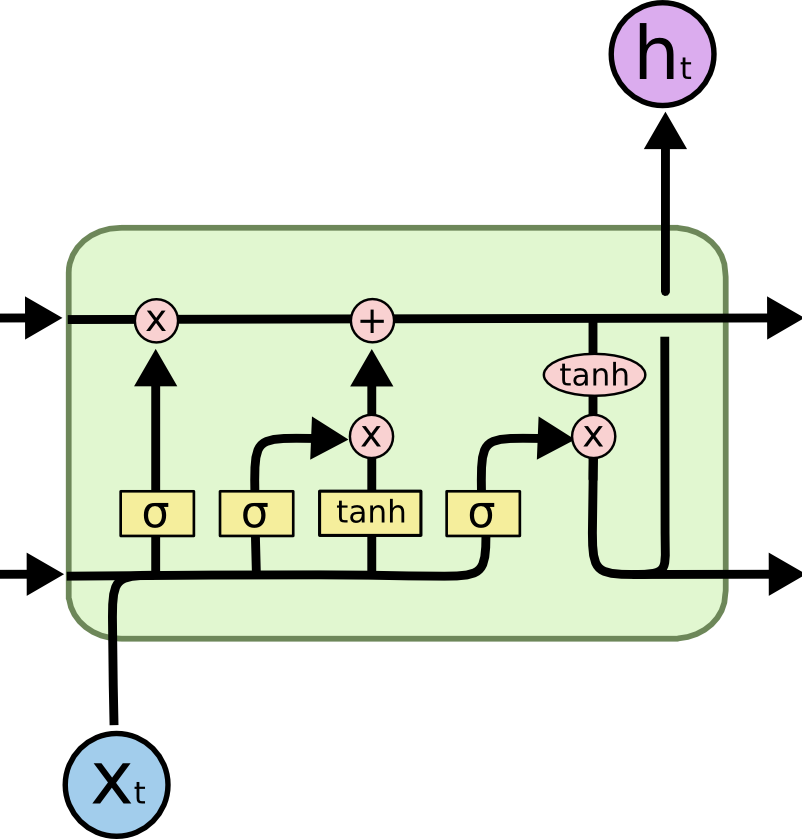
\includegraphics[scale=0.5]{figs/lstm_cell.png}
            \end{center}
            \caption{A single LSTM cell. From \cite{olah2015understanding}
            \label{fig:lstm_cell}}
        \end{figure}

        As can be seen in the Figure \ref{fig:lstm_cell}, there are quite a few more parameters in this cell than in a normal RNN cell. 
        The calculation of the output vector and the hidden vector involves several operations.
        First of all the network determines how much of the hidden state to forget, also called the forget gate. 
        This is done by pushing both the previous iteration's output ($c_{t-1}$) and the forget gate vector ($f_t$) through a matrix multiplication, allowing the network to forget values at specific indices in the previous iteration's output vector. 
        $f_t$ can be obtained by using formula in Equation \eqref{eq:forget_vector_lstm}, where $W$ contains the weights for the input and $U$ contains the weights for the previous iteration's output vector, $x_t$ refers to the input, $h_{t-1}$ to the previous iteration's output vector and $b$ is bias:
        \begin{equation}
            f_t = \sigma(W_f x_t + U_f h_{t-1} + b_f)
            \label{eq:forget_vector_lstm}
        \end{equation}

        The network then determines what to remember from the input vector.
        This, commonly referred to as the input gate, is done by pushing the previous forget gate's output as well as the input gate through a matrix addition. 
        The output of the input gate ($i_t$) can be found by using the following formula:

        \begin{equation}
            i_t = \sigma(W_i x_t + U_i h_{t-1} + b_i)
            \label{eq:input_vector_lstm}
        \end{equation}

        The final hidden state vector ($c_t$) can then be found by using the previous two results as follows:

        \begin{equation}
            c_t = f_t \circ c_{t-1} + i_t \circ \sigma(W_c x_t + U_c h_{t-1} + b_c)
            \label{eq:hidden_state_vector_lstm}
        \end{equation}

        where $\circ$ denotes the Hadamard product (where each value at index $ij$ is the product of the values at the indices $ij$ in the two input matrices).
        This vector is then passed on to the next iteration. 
        Now the output gate vector $o_t$ and the output state $h_t$ can be optained:

        \begin{align} 
            o_t &= \sigma(W_o x_t + U_o h_{t-1} + b_o) \label{eq:output_gate_lstm}\\
            h_t &= o_t \circ \sigma(c_t) \label{eq:hidden_output_gate_lstm}
        \end{align}

        This results in a version of an RNN that is able to remember more and is more liberal in choosing what information it wants to keep in the hidden state and what it wants to discard. 
        This makes LSTM networks better suited for tasks involving series of data and become the predominant RNN architecture. 

        \paragraph{Gated Recurrent Units} Another RNN architecture is the GRU, introduced in \cite{cho2014learning}. 
        This architecture combines the input and forget gates into a single so-called ``update gate'' and also merges the cell state and hidden state (see Figure \ref{fig:gru_cell}). 
        The calculation of the merged output vector once again consists of several operations.
        The network first computes the ``reset gate'' $r_t$ using the following function, where $W_r$ are the weights for the reset gate and $[h_{t-1}, x_t]$ signifies the concatenation of $h_{t-1}$ and $x_t$:

        \begin{figure}[h!]
            \begin{center}
                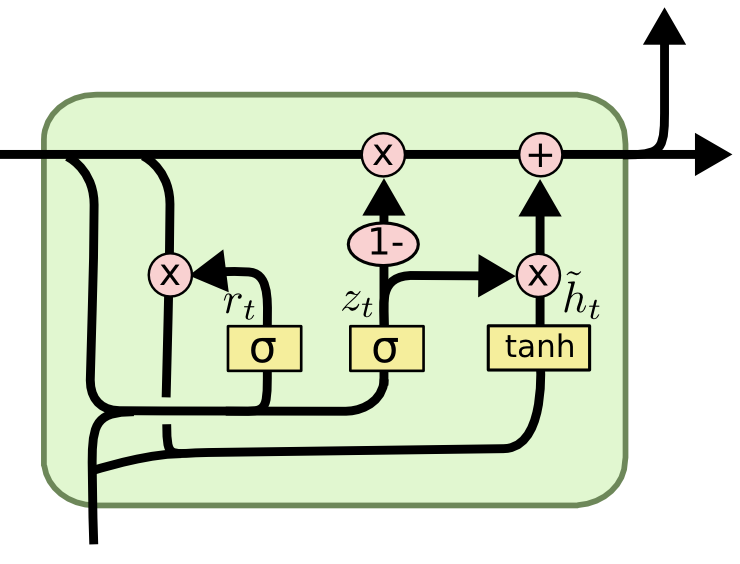
\includegraphics[scale=0.5]{figs/gru_cell.png}
            \end{center}
            \caption{A single GRU variation cell. From \cite{olah2015understanding}
            \label{fig:gru_cell}}
        \end{figure}

        \begin{equation}
            r_t = \sigma\left(W_r [h_{t-1}, x_t]\right)
            \label{eq:gru_reset_gate}
        \end{equation}

        After this, the ``update gate'' $z_t$ is computed as follows, where $W_z$ holds the weights of the update gate:

        \begin{equation}
            z_t = \sigma\left(W_z [h_{t-1}, x_t]\right)
            \label{eq:gru_update_gate}
        \end{equation}

        The output vector $h_t$ (representing both the cell's output and its state) can then be computed by the following formula:

        \begin{equation}
            h_t = (1 - z_t) * h_{t-1} + z_t * \tilde{h_t}
            \label{eq:gru_output}
        \end{equation}

        where $\tilde{h_t} = \tanh(W * [r_t * h_{t-1}, x_t])$.

        \paragraph{Bidirectional RNNs} It should be mentioned that when RNNs are used, they are often wrapped with a bidirectional layer.
        This simply reverts the input sequence and enters the sequence in both the original and the reverse direction to two separate RNNs, usually LSTM or GRU.
        % The usefulness of this is particularly intuitive when looking at the network in Figure \ref{fig:rnn}. 
        When processing the entry $x^{(j)}$, only the entries $t < j$ are known. 
        However, tokens later in the sequence might have an impact on the previous outputs of the model. 
        Bidirectional RNNs are able to capture patterns that are overlooked by regular RNNs.
